\usetikzlibrary{arrows.meta}

\begin{frame}{replace executable}
    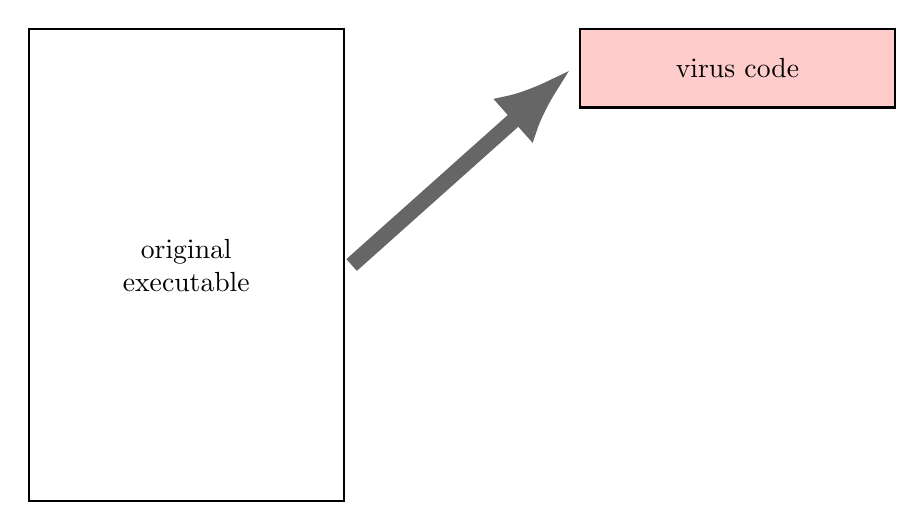
\begin{tikzpicture}
    \draw[thick] (0, 0) rectangle (4, -6) node[midway,align=center] {original\\executable};
    \draw[line width=2mm,-Latex,black!60] (4.1, -3) -- (6.9, -.5);
    \begin{scope}[xshift=7cm]
    \draw[thick,fill=red!20] (0, 0) rectangle (4, -1) node[midway,align=center] {virus code};
    \end{scope}
    \end{tikzpicture}
\end{frame}

\begin{frame}{replace executable?}
    \begin{itemize}
    \item seems silly --- not stealthy!
    \item has appeared in the wild --- ILOVEYOU
    \item 2000 ILOVEYOU Worm
        \begin{itemize}
        \item written in Visual Basic (!)
        \item spread via email
        \item replaced lots of files with copies of itself
        \end{itemize}
    \item huge impact --- because destroying data to copy itself
    \end{itemize}
\end{frame}

\begin{frame}{replace executable --- subtle}
    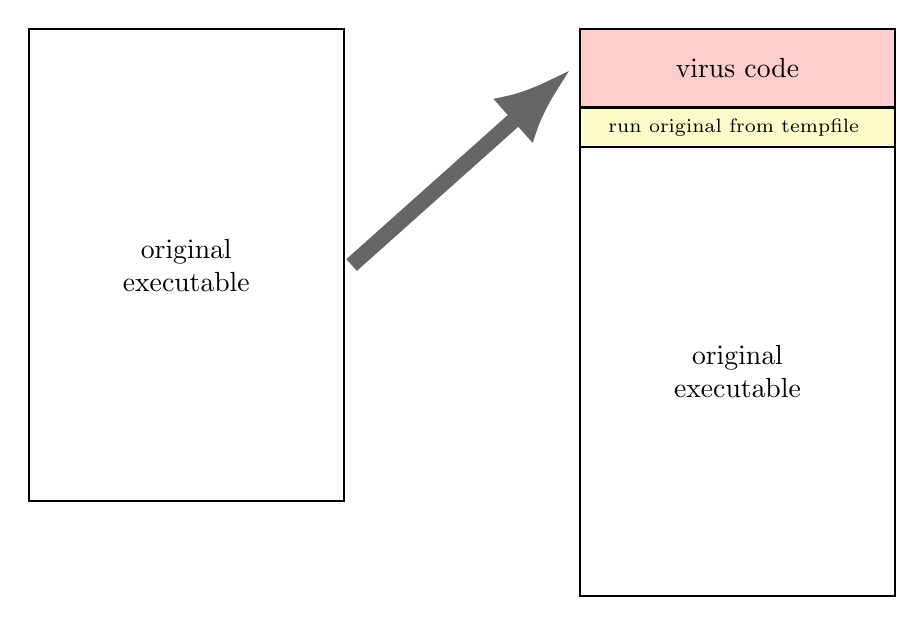
\begin{tikzpicture}
    \draw[thick] (0, 0) rectangle (4, -6) node[midway,align=center] {original\\executable};
    \draw[line width=2mm,-Latex,black!60] (4.1, -3) -- (6.9, -.5);
    \begin{scope}[xshift=7cm]
    \draw[thick,fill=red!20] (0, 0) rectangle (4, -1) node[midway,align=center] {virus code};
    \draw[thick,fill=yellow!20] (0, -1) rectangle (4, -1.5) node[midway,align=center,font=\scriptsize] {
        run original from tempfile
    };
    \draw[thick] (0, -1.5) rectangle (4, -7.2) node[midway,align=center] {original\\executable};
    \end{scope}
    \end{tikzpicture}
\end{frame}

